\documentclass[./FinalReport.tex]{subfiles}

%Bezier Extraction
\begin{document}
B\`{e}zier extraction, discussed at length in \cite{borden_isogeometric_2011} fundamentally links the the NURBS basis technology of IGA with the data structures prevalent in classical Finite Elements. As illustrated above, B-spline bases (and NURBS) have support spanning several elements (knot spans). This extended support is partially responsible for the improved accuracy of IGA over typical Finite element methods, though it is also fundamentally incompatible with current discretization technologies widely employed for performing Finite Element Analysis. Specifically, classical Finite elements relies on a straightforward pull back from an element in the parametric domain to a parent element. This mapping is simple because typical bases utilized in classical Finite Elements are designed strictly with local support over an element in parametric space. This presents a problem for our bases derived from B-spline technology, as B-splines and NURBS do not have local support, we would have to store information about each basis over every element in the domain. Fortunately, through the extraction operator, we may represent B-spline bases as a linear combination of Bernstein bases with local support over each element (knot span). This mapping is performed through the \textit{extraction operator}. 

The extraction operator maps Bernstein polynomials to B-spline bases via a simple linear combination.  As such, a single Bernstein parent element can be employed to integrate B-spline bases into a typical Finite Element data structure. These two sets of bases are shown side by side in Figure \ref{fig:extracted}. This operator is constructed by mapping the effect of increasing the multiplicity of each knot through the interior of the domain until high order continuity of the bases is broken across knots, leaving $C^0$ continuous bases across knots. This expanded basis becomes Bernstein polynomials over each knot span. The effect of knot insertion is stored in matrix form in the extraction operator. 

\begin{figure}
  \centerline{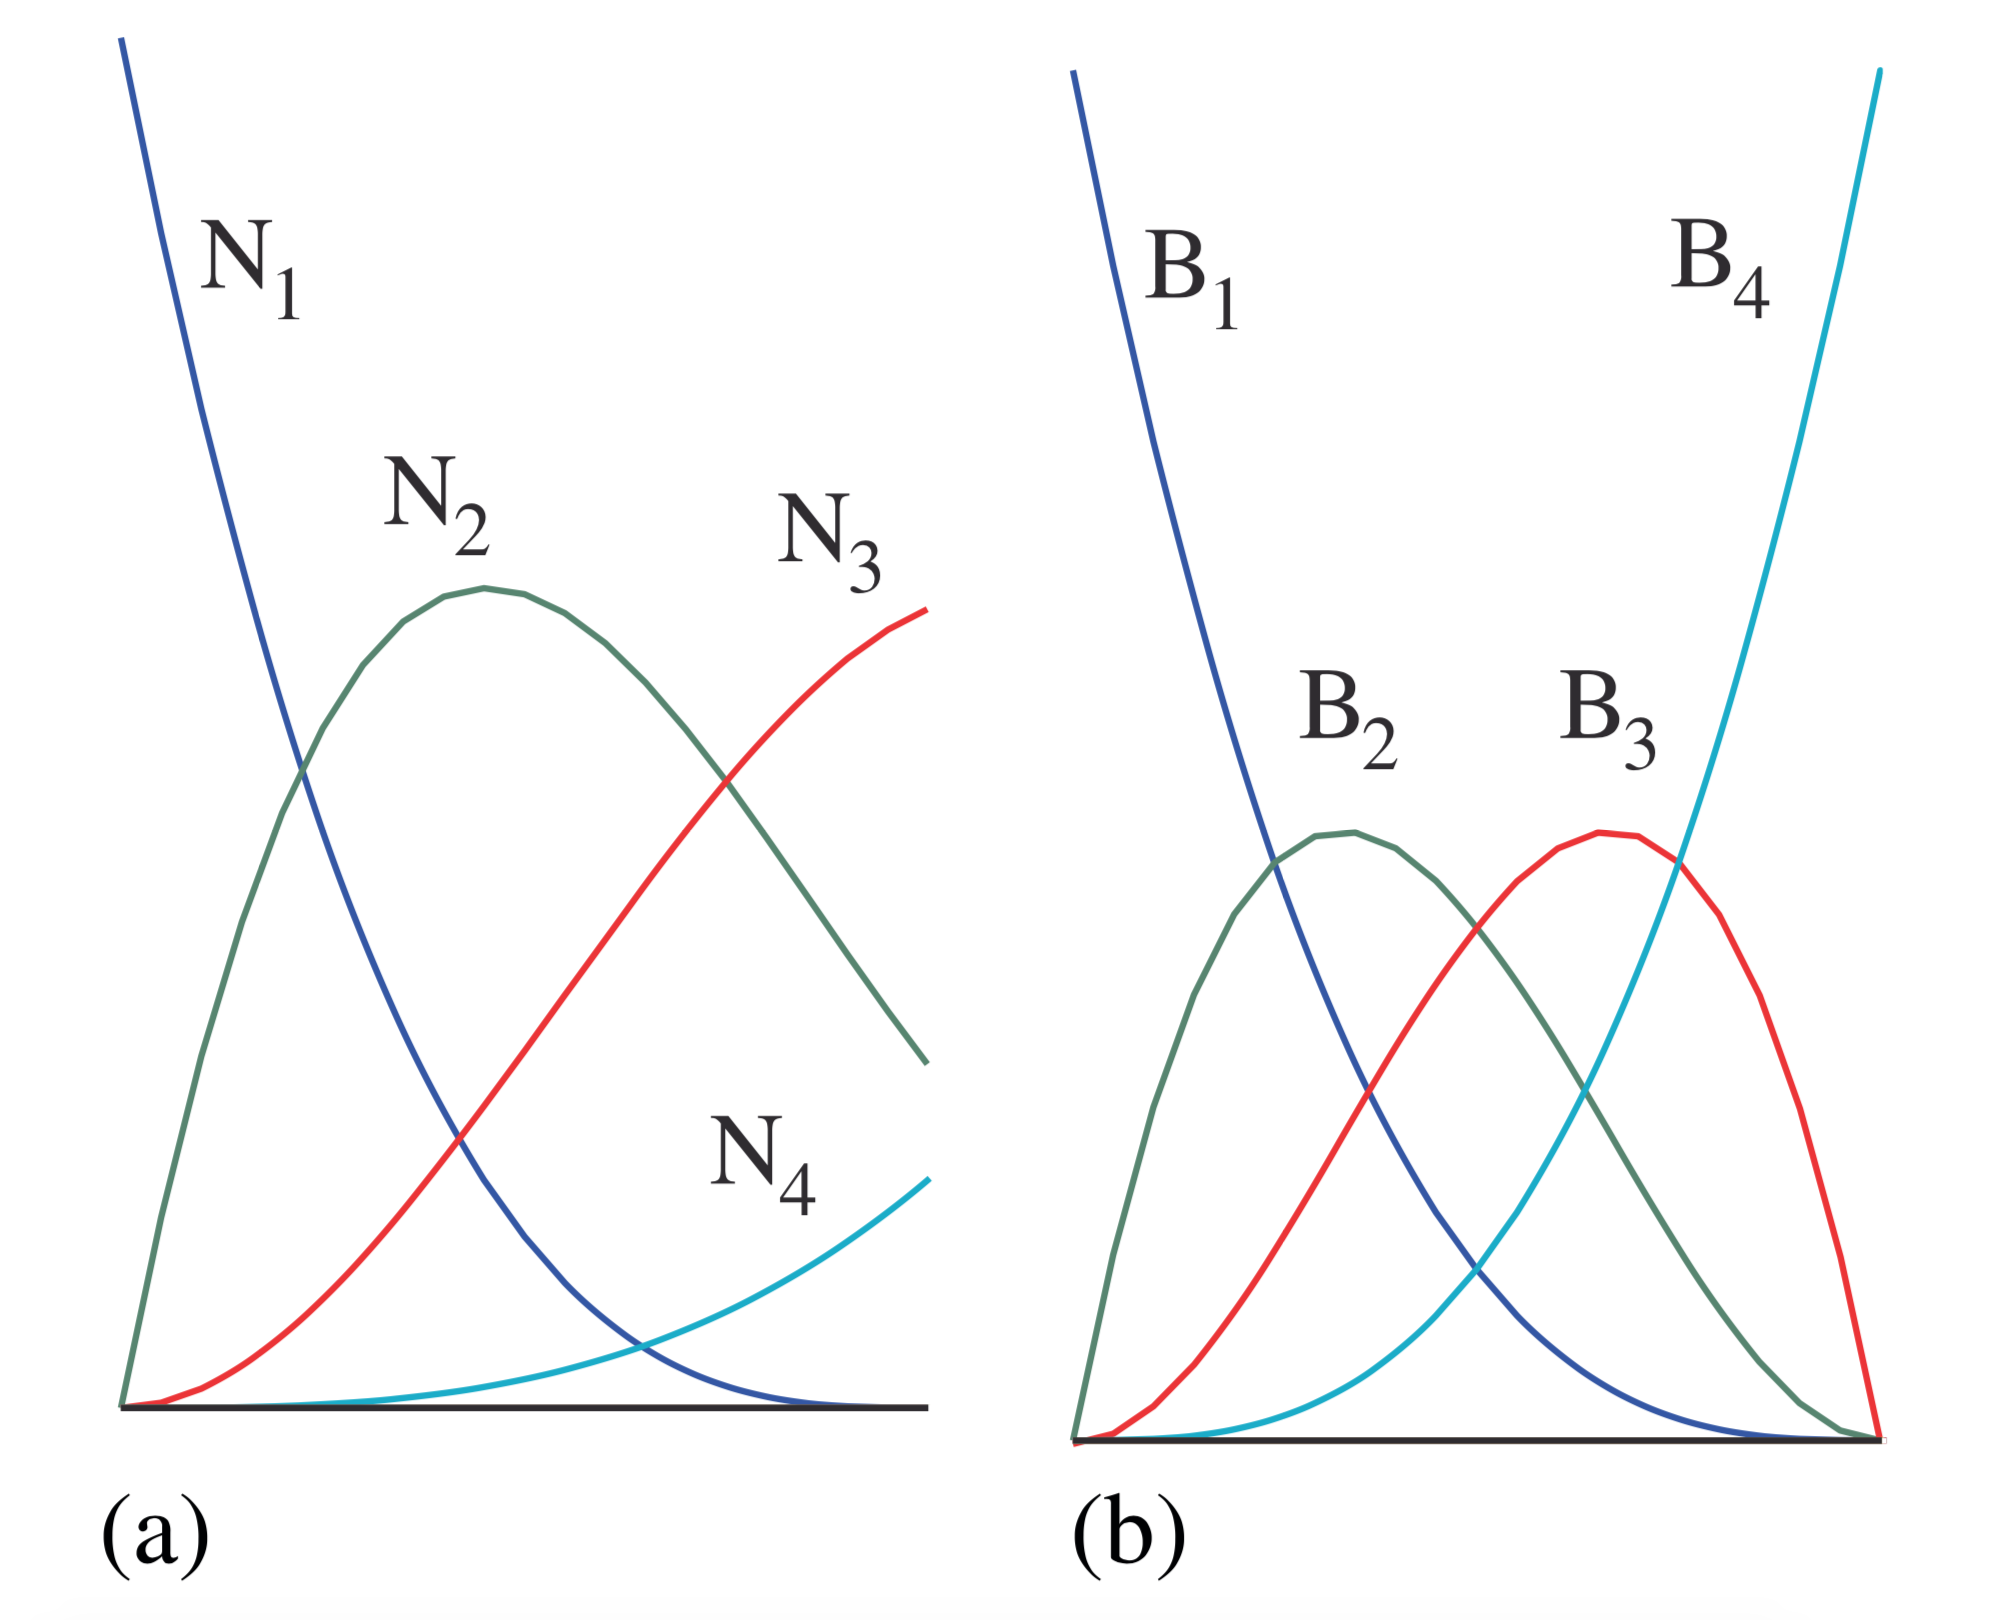
\includegraphics[width=4in]{./figures/Extracted_B-Spline}}
  \caption{\cite{borden_isogeometric_2011} B-Spline bases over a knot span (as in (a), $[0,1]$) can be written as linear combination of Bernstein bases (b) over their unit domain. The extraction operator stores the coefficients of these linear combinations.}
  \label{fig:extracted}
\end{figure}

B\`ezier extraction is possible over NURBS bases as well by projecting the NURBS bases onto a set of B-spline bases one dimension higher \cite{piegl_nurbs_2012}. 
\end{document}